\chapter{机器学习方法预估震级效果评估与讨论 }
\section{数据分析与预处理}
\indent 利用第二、三章所描述的方法,本文搭建并实现了$\tau_{c}$方法和机器学习类模型进行效果检验。考虑到震级紧急预估的应用场景和所需要的基础设施需求,我们将研究区域定位日本岛区域。原始全数据集使用了日本KIK和KNET两台站网从2015至2017年所记录到的所有大于3级且震源靠近日本岛主体的地震记录,除此之外并无经过其他任何的主动事件挑选,事件分布如下图4.1所示。\\
\begin{figure}[!h] 
\centering 
 \includegraphics[width=0.8\linewidth]{img/basemap.jpg} 
 \renewcommand{\figurename}{图} 
\caption{全数据集地震事件} 
%英文标题begin 
\addtocounter{figure}{-1} \vspace{-5pt} 
%\SetEnglishCaption 
\renewcommand{\figurename}{Fig} 
\caption{Full data set earthquake event} 
\renewcommand{\figurename}{图} 
%英文标题end 
\label{fig:network-device-influence.png} 
\end{figure}
\indent 原始全数据中共包含了840个地震事件,合计50314条记录,具体的分布和统计如下图4.2和4.3所示,其中包含了3级至4级地震事件共420个、10145条地震台站记录,4级至5级地震事件共216个、14629条地震台站记录,5级至6级地震事件共61个、10740条地震台站记录,6级以上地震事件共8个、1004条地震台站记录。\\
\begin{figure}[!h] 
\centering 
 \includegraphics[width=0.95\linewidth]{img/Event distribution.png} 
 \renewcommand{\figurename}{图} 
\caption{全数据集地震事件} 
%英文标题begin 
\addtocounter{figure}{-1} \vspace{-5pt} 
%\SetEnglishCaption 
\renewcommand{\figurename}{Fig} 
\caption{Full data set earthquake event} 
\renewcommand{\figurename}{图} 
%英文标题end 
\label{fig:network-device-influence.png} 
\end{figure}
\indent 图5(a)显示了不同震级的地震数目分布。总体来看震级分布十分不均匀,小地震远多于大地震。但大地震破坏力大危害深重是我们在紧急预警系统中容错率低的部分,其在原始分布中、在训练集中出现频率低,不利于模型学习到关于如何预估大型地震震级的规则,给模型的训练带来较大的困扰。我们采取在训练集中对大地震数据过采样再加一定噪音的方法,以此处理数据分布不平衡问题。将原始的如图5(a)分布修正为图5(b),一定程度上缓解该问题。\\
\begin{figure}[!h] 
\centering 
 \includegraphics[width=0.95\linewidth]{img/event_dist.png} 
 \renewcommand{\figurename}{图} 
\caption{数据集中地震记录的震级分布。横轴为震级$\mathbf{M}_{\mathbf{w}}$,纵轴为该震级的台站记录数目。\\
(a) 原始分布;(b) 调整后分布} 
%英文标题begin 
\addtocounter{figure}{-1} \vspace{-5pt} 
%\SetEnglishCaption 
\renewcommand{\figurename}{Fig} 
\caption{Magnitude distribution of seismic records in data sets, The horizontal axis is the magnitude $\mathbf{M}_{\mathbf{w}}$, and the vertical axis is the number of stations recorded for this magnitude.\\
(a) Original distribution; (b) Adjusted distribution
} 
\renewcommand{\figurename}{图} 
%英文标题end 
\label{fig:network-device-influence.png} 
\end{figure}


\section{不同方法的评估比较}
\indent 训练曲线如图6所示,两条图线分别为训练数据集和交叉数据集的均方根误差(RMSE)随着训练步数的变化。在经过NN模型经过大约150000步训练后,虽然训练数据集级上模型表现持续变好,但在交叉检验数据集上RMSE停止减小并开始增大,触发提前停止条件(Early Stopping)。故在此训练步数上停止训练,并存储此时的模型最佳权值。\\
\begin{figure}[!h] 
\centering 
 \includegraphics[width=0.8\linewidth]{img/6.eps} 
 \renewcommand{\figurename}{图} 
\caption{NN模型训练曲线。横轴为训练步数,纵轴为均方根误差(RMSE)。} 
%英文标题begin 
\addtocounter{figure}{-1} \vspace{-5pt} 
%\SetEnglishCaption 
\renewcommand{\figurename}{Fig} 
\caption{NN Model training curve. The horizontal axis is the number of training steps and the vertical axis is the root mean square error (RMSE).} 
\renewcommand{\figurename}{图} 
%英文标题end 
\label{fig:network-device-influence.png} 
\end{figure}
\indent 在图7和8中我们还原Kanamori (2008)的$\tau_{\mathrm{c}}$方法(以下简称为“K方法”),并使其与NN模型在同样的测试数据集上相比较。在图(7)中可发现如果和K方法一样,考察震级大于4级情况,NN模型和K方法的RMSE分别为0.29和0.59,NN模型具有优势。图7(a) K方法的结果中的实线为拟合$\tau_{\mathrm{c}}$和$\mathrm{M}_{\mathrm{w}}$的线性关系,实线上下两条虚线代表了一个平均标准差的范围。图中的小正方形为多台站联合预估震级的平均结果,而方框上下的延长线为该事件的一个标准差的置信区间。如果把最小震级的限制从4级扩展到更为广泛的3级,如图8所示,NN模型和K方法的RMSE分别为0.51和1.06。\\
\begin{figure}[!h] 
\centering 
 \includegraphics[width=\linewidth]{img/7.eps} 
 \renewcommand{\figurename}{图} 
\caption{单一事件预估方差分布。横轴为方差大小,纵轴为该方差的密度。\\
(a) 采用Kanamori et al. (2008)方法的结果,纵轴为K方法的$\log \left(\tau_{\mathrm{c}}\right)$;(b) NN模型的结果,纵轴为机器学习模型给出的预估震级} 
%英文标题begin 
\addtocounter{figure}{-1} \vspace{-5pt} 
%\SetEnglishCaption 
\renewcommand{\figurename}{Fig} 
\caption{The magnitude prediction effect is compared (minimum magnitude 4) and the horizontal axis is the real magnitude.\\
(a) Using the results of Kanamori et al. (2008), the vertical axis is the $\log \left(\tau_{\mathrm{c}}\right)$ of the K method; (b) the result of the NN model, the vertical axis is the predicted magnitude given by the machine learning model.} 
\renewcommand{\figurename}{图} 
%英文标题end 
\label{fig:network-device-influence.png} 
\end{figure}


\begin{figure}[!h] 
\centering 
 \includegraphics[width=\linewidth]{img/8.eps} 
 \renewcommand{\figurename}{图} 
\caption{ 震级预估效果对比(最小震级3级)。横纵坐标同图4.4。\\
(a) 采用Kanamori et al. (2008)方法的结果;(b) NN模型的结果} 
%英文标题begin 
\addtocounter{figure}{-1} \vspace{-5pt} 
%\SetEnglishCaption 
\renewcommand{\figurename}{Fig} 
\caption{The magnitude of the earthquake prediction results (minimum magnitude 3). \\
The horizontal and vertical coordinates are the same as in Figure 4.4.
(a) Results using Kanamori et al. (2008) (b) The results of NN model
} 
\renewcommand{\figurename}{图} 
%英文标题end 
\label{fig:network-device-influence.png} 
\end{figure}


\indent 图9显示了对单一事件两种方法的预估方差情况。可以看出,不仅对于整体预估效果而言,NN模型预估方差小。并且从单一事件多台站的方差分布角度来看,NN模型的方差分布在两种最低截至震级模型下都更为左移,也表明模NN型的稳定性优于Kanamori(2008)的$\tau_{\mathrm{c}}$方法。
\begin{figure}[!h] 
\centering 
 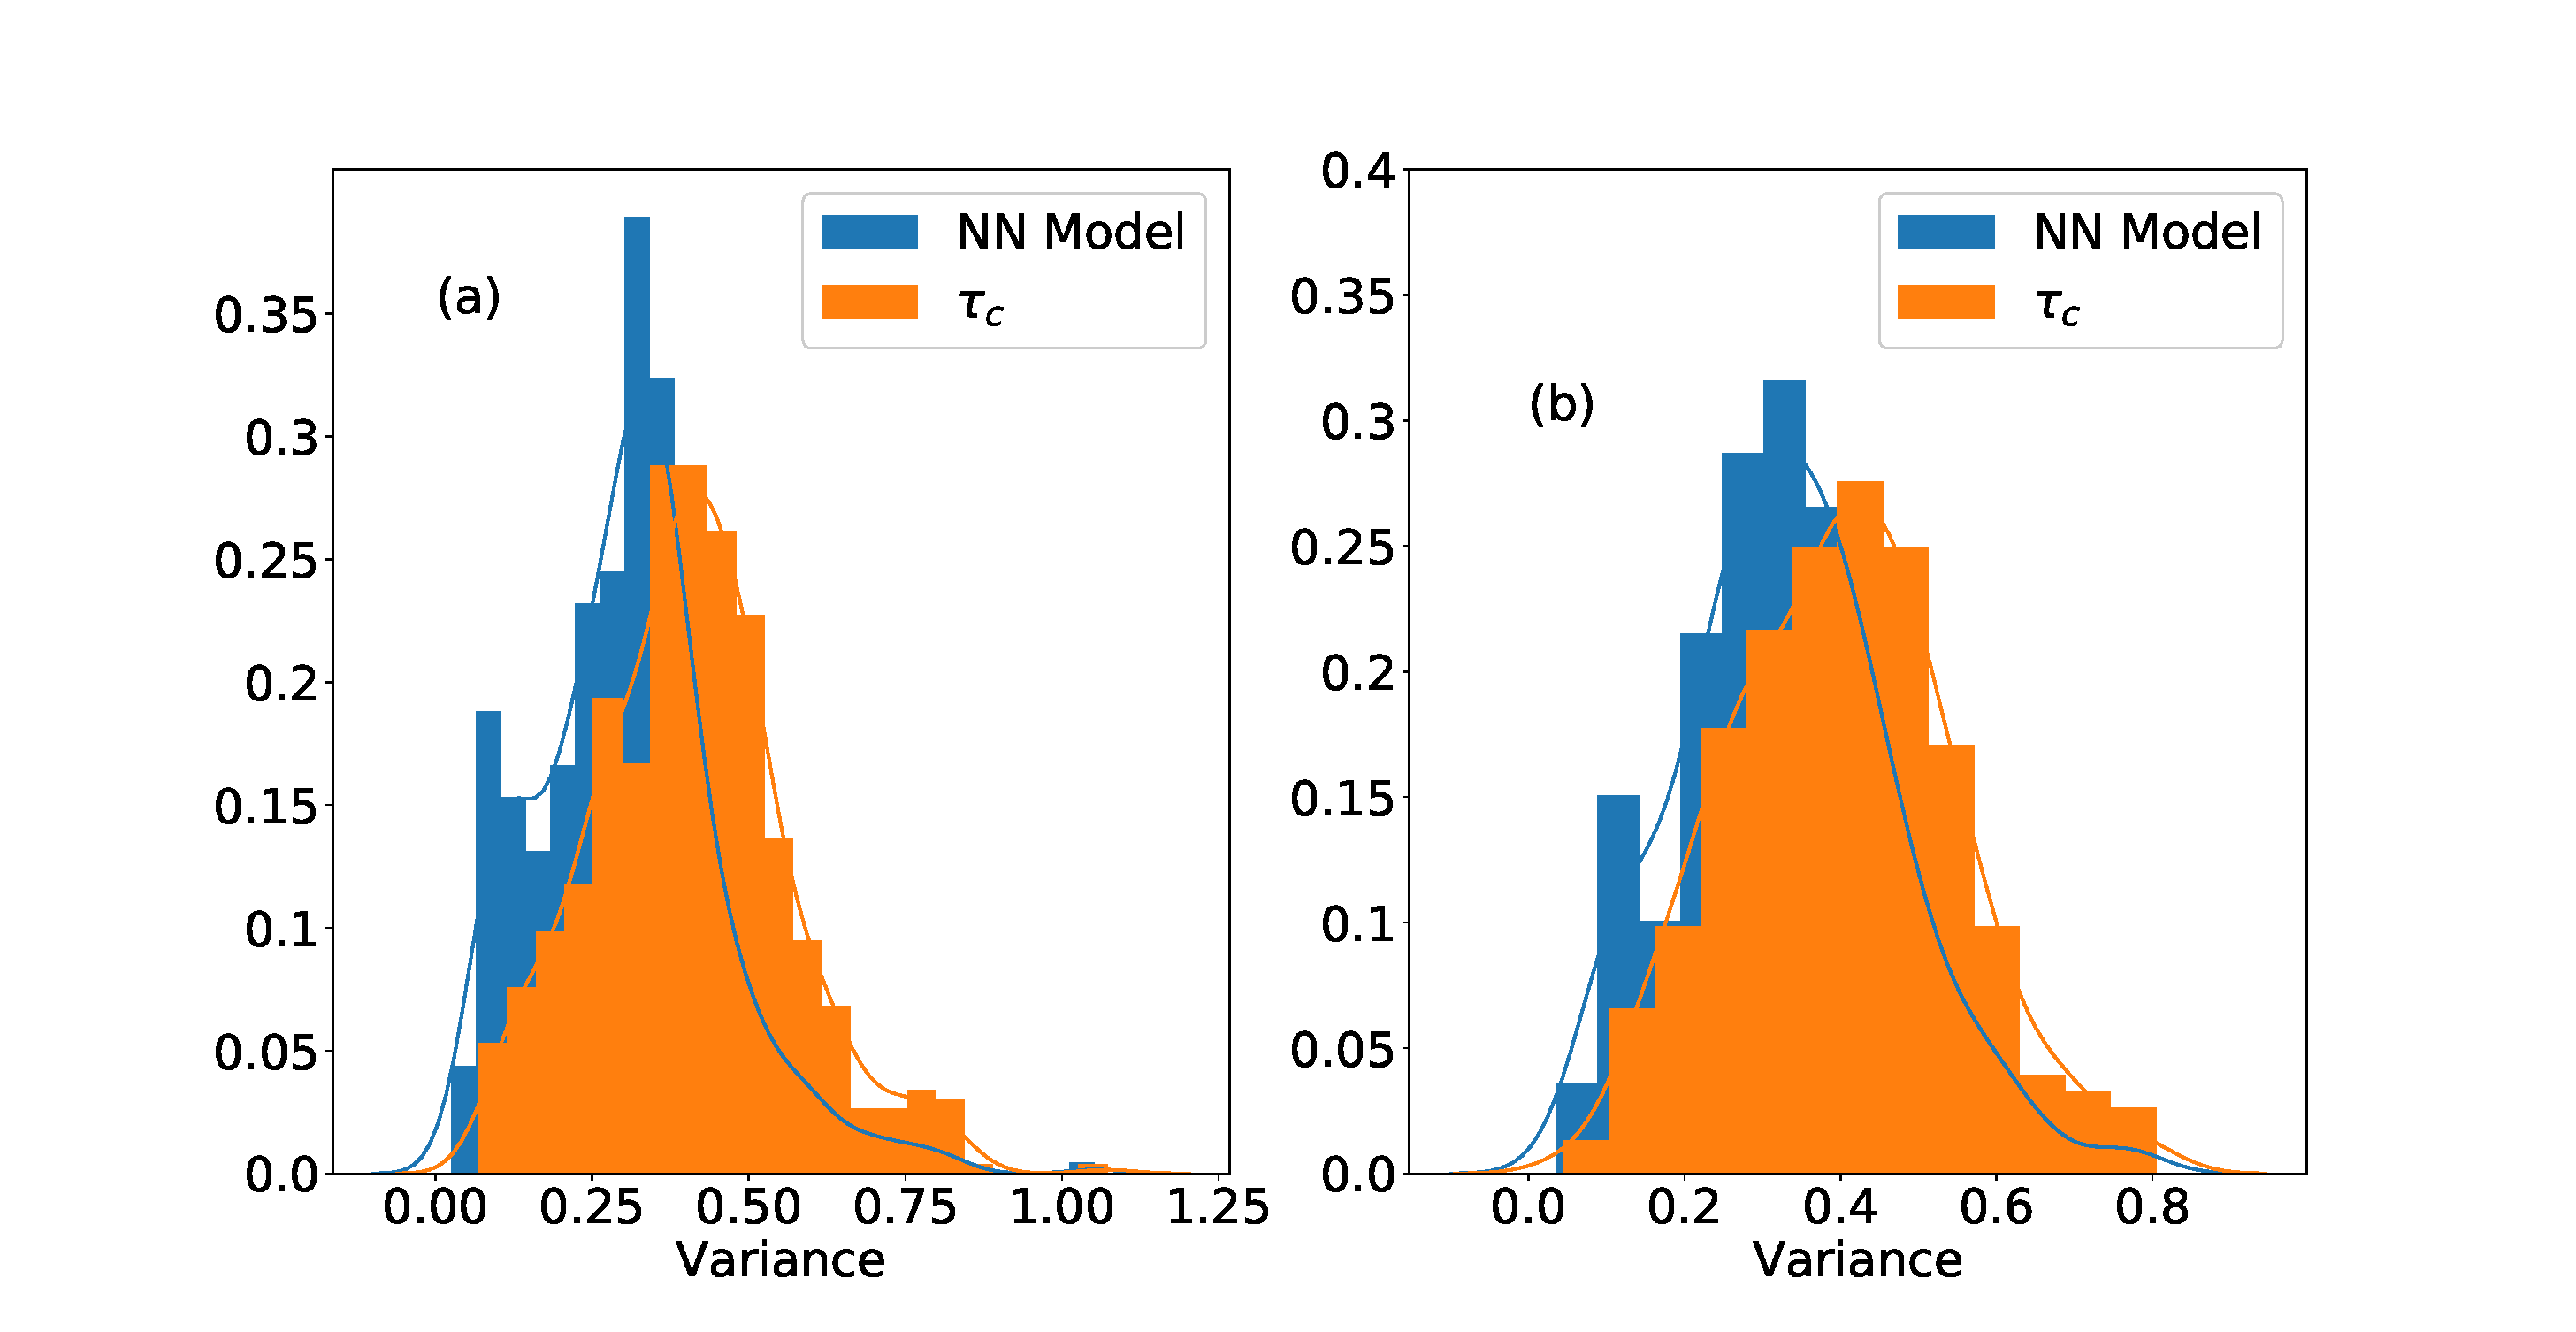
\includegraphics[width=\linewidth]{img/9.eps} 
 \renewcommand{\figurename}{图} 
\caption{单一事件预估方差分布。横轴为方差大小,纵轴为该方差的密度。\\
(a) 截至震级为4级K方法与NN模型方差分布;\\
(b) 截至震级为3级K方法与NN模型方差分布} 
%英文标题begin 
\addtocounter{figure}{-1} \vspace{-5pt} 
%\SetEnglishCaption 
\renewcommand{\figurename}{Fig} 
\caption{Single event estimation variance distribution. The horizontal axis is the variance and the vertical axis is the density of the variance.\\
(a) The Kanamori method and the NN model variance distribution up to the
magnitude 4; \\
(b) The Kanamori method and the NN model variancedistribution up to the magnitude 3} 
\renewcommand{\figurename}{图} 
%英文标题end 
\label{fig:network-device-influence.png} 
\end{figure}